% !TEX root = ./skripsi.tex
\chapter{INTRODUCTION}
\section{Background}\label{sec:background} %pelabelan ini opsional, biar bisa di klik kalo mengarahkan ke section tertentu.
\noindent Partial differential equations (PDE) are a common tool widely used in the modern scientific understanding and many engineering processes. This is because many systems can be described by the way they change and often this can be more intuitive. As an example, think of someone heating up a large frying pan on a gas stove. To describe how the pan heats up when the center is right above the burner, one can say that the center would heat up first followed by its surroundings. Eventually the pan would not heat up any further. Also notice that the edges of the pan would always be cooler than the center. However, once a more complex setup is introduced such as an uneven heat source or more complex materials with different heat rates of transferring heat it becomes much harder to describe how the pan heats up. A more useful way to describe the system is using the heat equation. For a temperature function \(u\left(\vb{x},t\right)\) of spatial coordinates vector \(\vb{x}\) and time \(t\), the generalized heat equation is defined in \lccref{eq:heat_equation}.
\begin{equation} \label{eq:heat_equation}
    \pdv{u}{t}=\divergence{\left(\alpha \gradient u\right)}
\end{equation}
The divergence operator \(\divergence \) denotes sum of all first spatial derivatives. In three dimensions this is \(\divergence=\pdv{\cdot}{x_1}+\pdv{\cdot}{x_2}+\pdv{\cdot}{x_3}\). And the gradient operator \(\gradient \) is the vector of all first spatial derivatives which in three dimensions is \(\gradient{f} = {\begin{bmatrix}\pdv{f}{x_1} & \pdv{f}{x_2} & \pdv{f}{x_3}\end{bmatrix}}^{\intercal}\). This equation says that the rate at which the temperature changes in time \(\pdv{u}{t}\) is proportional to how different the differences in temperature of a spot in the pan with its surroundings \(\laplacian{u}\) multiplied with thermal diffusivity parameter \(\alpha \). One example of an insight this gives is that given a homogeneous material (\(\alpha \) is constant) and the stove outputs heat at a constant rate the temperature will no longer change for a particular point once the temperature difference is constant. In other words once the function \(u\left(\vb{x},t\right)\) at some time \(t > 0 \) approaches a linear function in space, the temperature at all spots will no longer change in time. Mathematically this is because the time derivative is zero if the second spatial derivatives are also zero. Intuitively this is because once the temperature distribution approaches linear, the current spot on the pan is outputting as much heat it is getting. This insight is an example of why PDEs are useful.

Many other fields in physics such as waves, quantum dynamics, fluid dynamics, elastics, and many more also define systems using PDEs. PDEs are also used outside the physical sciences. In Finance, the Black-Scholes-Merton or Black-Scholes equation models the dynamics of the financial market. In ecology, PDEs are used to model population growth which is useful for modelling location dependent carrying capacity. This is used to model species distribution which can help develop better conservation policies. In the social sciences, PDEs such as the cross-diffusion model is used to explore the evolution of the urban environment \autocite{jinDetectingInteractionUrban2023}. Crowd dynamics is another field where researchers have found it useful to model using PDEs \autocite{mukherjeeLagrangianApproachModeling2015,hughesFlowLargeCrowds2000}. These are used to model dynamics such as shock-waves, pathing, and crowd flow as a whole. There are a variety of applications, ranging from bird flocks, pedestrian crowds, to robotic swarms \autocite{gongCrowdDynamicsModeling2023}.

An increasingly critical use of PDEs is in Numerical weather prediction (NWP). The information weather forecasts provide is an integral part of modern life. Many sectors rely on timely and accurate weather forecasts. Individuals, day to day rely on forecasts for a range of different decisions ranging from activities they can do to personal safety from extreme weather. The weather also affects retail as consumer behavior change with whether it is rain or shine \autocite{tianImpactWeatherConsumer2021,tianPredictingConsumerVarietyseeking2018,govindWeatherAffectPreference2020,moonWeatherSensitivityAnalysis2018}. Similarly, the types of transportation people use and operational decisions changes with the weather \autocite{lepageImpactWeatherActivities2021,nurmiExpectedImpactsValue2013}. Another critical sector is agriculture, where extreme weather events and changes in climate threatens the food supply \autocite{cogatoExtremeWeatherEvents2019,malhiImpactClimateChange2021,anwarAdaptingAgricultureClimate2013}. As the climate continues to warm and extreme weather events increase in frequency, the mitigation for these events become all the more important \autocite{ClimateChange20222023}. Because of this, forecasting is critical in making accurate decisions for policymakers and warnings of extreme weather events for civilians \autocite{astithaExtremeWeatherForecasting2023,stottAttributionExtremeWeather2016}. A major challenge is the fact that observations of weather can be sparse in the sense that observations are localized and do not cover entire areas \autocite{wilbyRainfallTemperatureEstimation2013,monmonierAirApparentHow1999,galkinAssimilationSparseContinuous2020}. This lack of spatially distributed meteorological information hampers decision-making on areas to be prioritized and what to prioritize based on location. For example, weather stations can only observe their immediate surroundings. And they are for the most part stationary. Even more mobile observation platforms like satellites only show the portion of the surface the satellite can see at any one time such as in \lccref{fig:satellite_image_coverage}. While accumulating observations through more satellite passes is possible, this, however, means short-lived features may not be observed. As impoverished regions often are the most data sparse, the effect compounds on the fact that for impoverished regions, scarce resources need to be effectively and efficiently applied. To this end, numerical models are employed to model a more representative view by using known physics such as the compressible Euler equations and statistical models \autocite{mengaldoCurrentEmergingTimeIntegration2019,kwasniokDatabasedStochasticSubgridscale2012}. The next step is in forecasting future weather which in itself is a challenge. The information this could provide is invaluable because it means planning for future weather is possible.

\begin{figure}[h] %h means here!
    \centering
    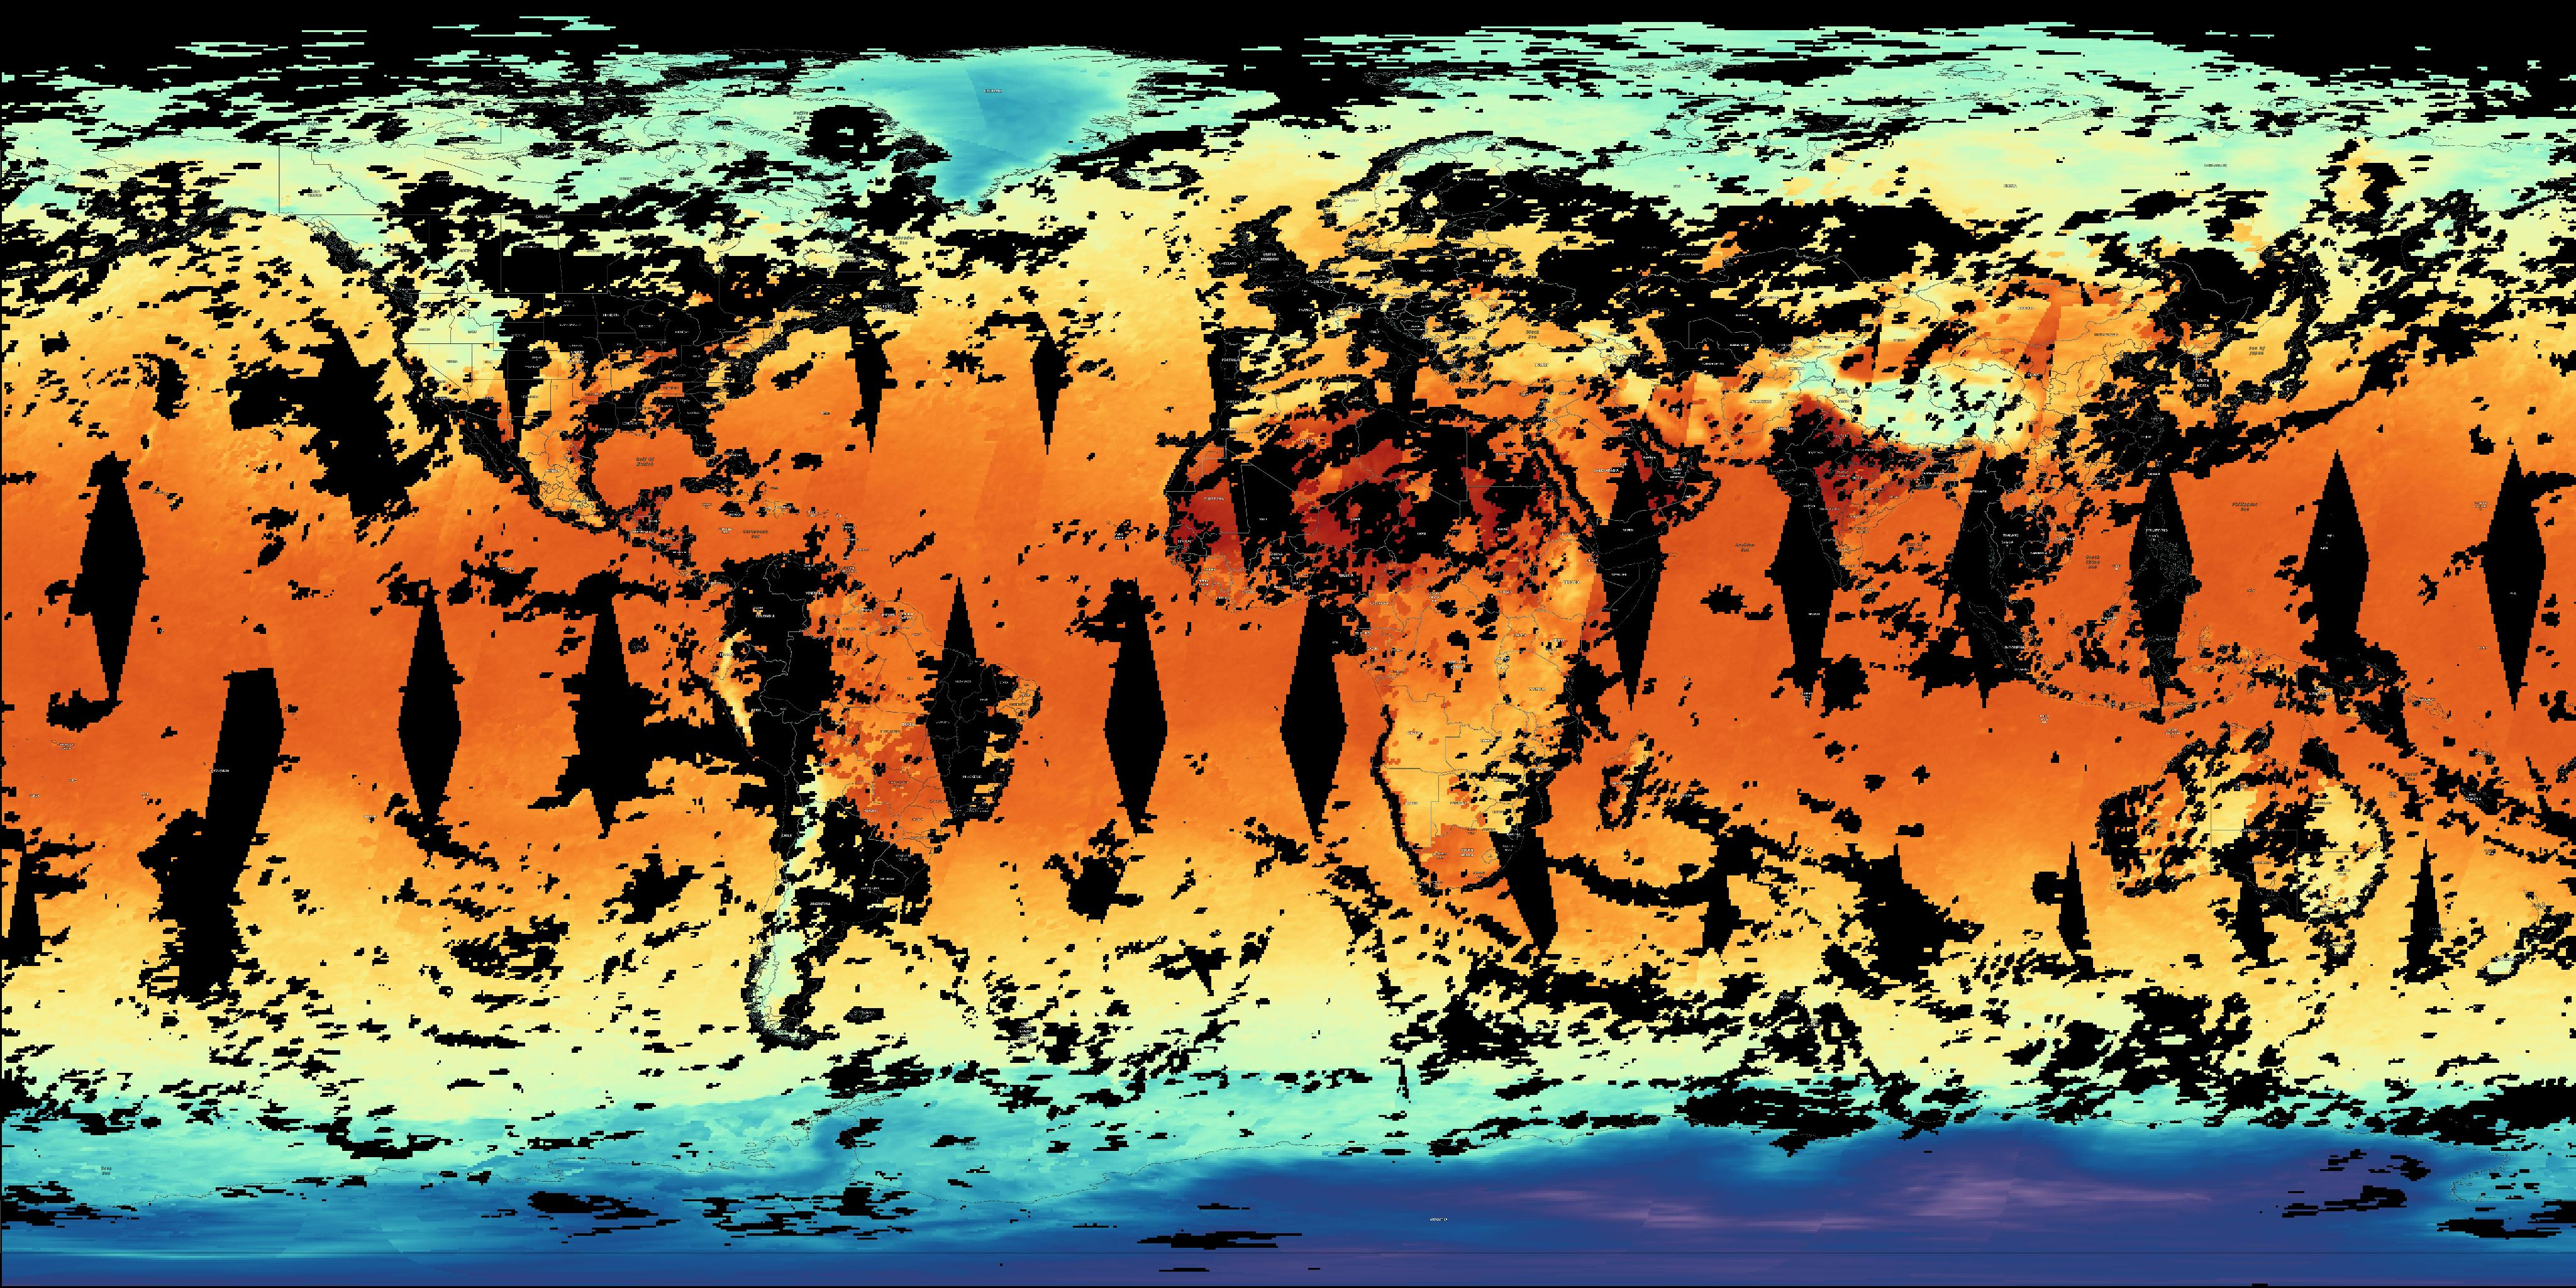
\includegraphics[width=1.0\linewidth]{figures/snapshot_nasa_airs_aqua_2024_05_21T00_00_00Z.jpg}
    \caption{Daytime and nighttime surface air temperature from observations by the AIRS instrument onboard the NASA AQUA satellite. This shows observations recorded through a whole day on the 21\textsuperscript{st} of May 2024. Notice that parts of the globe, especially near the equator have not been observed. This image was produced using NASA Worldview (\url{https://go.nasa.gov/46SaYyJ}).}\label{fig:satellite_image_coverage}
\end{figure}

Forecasting the weather or evolution of any other system is formulated as an initial value problem where past observations are used to predict an unknown future state of the system. A different formulation can be how heat spreads over time in different types of frying pans from known information of the pan's materials, their heat conduction properties, and that the stove gives off constant heat. In general the scenario is predicting the effect (future atmospheric temperature distribution, etc.) of some given causes (current and past weather, etc.). This scenario is termed the forward problem. The inverse problem on the other hand solves for an unknown parameter using other known parameters and observations of the partial solution such as temperature field at the object's surface. Traditional methods used to solve these problems utilized knowledge of the exact equations to numerically solve PDEs. As an example, the Finite Difference Method (FDM) approximates the solution by substituting the partial derivatives with finite differences and manipulating the equation such that the solution can be computed. The inverse problem on the other hand is determination of initial conditions or other parameters from observed state of the system. For example determining the heat source distribution given the temperature distribution at some point in time. One traditional approach to this would have meant solving the forward problem from an initial guess of the parameter and then evaluating some cost function such as how close the predicted solution is to the observed one. As expected, this would require many evaluations of the forward solver. This means that the cost of the solver would be greatly multiplied, emphasizing the importance of an efficient solver.
% TODO: reword this because the explanation of the problem setup for forward and inverse problems is not layed out optimally.
% TODO: perhaps the disadvantage of inverse problem in the paragraph above should be removed and only explanation of the inverse problem setup itself left by itself
% \begin{equation} \label{eq:forward_finite_difference_1}
%     \pdv{f\left(x\right)}{x} \approx \frac{f\left(x+h\right)-f\left(x\right)}{h}
% \end{equation}

Traditional numerical solvers have enjoyed many decades of development due to their long history. There are many general approaches to solve PDEs and many more very specific approaches. Other than FDM, some widely used approaches include Finite Element Methods (FEM), Finite Volume Methods (FVM), Collocation Methods, and Spectral Methods. FEM and FDM are both mesh based approaches, meaning they rely on discretization of the computational domain. There are several challenges associated with this. First, irregular domains such as bio-inspired materials like bone, spider silk, or aggregate materials like gravel pose a challenge due to the complexity of the domain geometry \autocite{gaulSimulationWavePropagation1991,buoniEfficientScalableNumerical2007,jiaModulateStressDistribution2024}. Also, irregular domains which create large deformations or mesh entanglement cause these methods to become ineffective \autocite{chenMeshfreeMethodsProgress2017}. While there are strategies to mitigate this, by definition they are an additional layer of difficulty to the process. Second, multiscale applications where the micro and macro scales are both important require fine meshes such that the small scale structures are adequately simulated. This creates meshes with very large number of points that are very resource intensive \autocite{buoniEfficientScalableNumerical2007}. Third, a single evaluation of traditional mesh-based solvers may not be very costly, however multiple evaluations can add up. This is very apparent in inverse problems where the solver is queried multiple times to solve the forward problem in order to obtain parameter functions. Therefore, in problems where these issues important or resources are limited, mesh-free methods may be preferred. As an example, the spectral method solves PDEs by formulating the solution as a linear combination of global basis functions like the Fourier series. This can be likened to how music combines sound waves of different things to produce the overall sound. The complex formulation of the Fourier series is presented in \lccref{eq:fourier_series}.
% TODO: Add diagram example for discretization of the domain by FEM/FDM methods
\begin{equation}\label{eq:fourier_series}
    s = \sum_{k} c_k e^{2\pi ikx}
\end{equation}
The example differential equation we wish to solve is the simple derivative in \lccref{eq:derivative}. In other words, the aim is to find a function \(u^{*} \) from a known function \(f^{*} \). This means we are learning the anti-derivative operator or more loosely known as the integral. To do this we first formulate both into separate Fourier series approximations \(u \) and \(f \) in \lccrefs{eq:example_fourier_1,eq:example_fourier_2} respectively.
\begin{align}
    \dv{u^*\left( x \right)}{x} & = f^*\left( x \right) \label{eq:derivative}                                                      \\
    u^*\left( x \right)         & \approx u\left( x \right)         = \sum_{k} \hat{u}_k e^{2\pi ikx} \label{eq:example_fourier_1} \\
    f^*\left( x \right)         & \approx f\left( x \right)         = \sum_{k} \hat{f}_k e^{2\pi ikx} \label{eq:example_fourier_2}
\end{align}
Next we take the derivative of \lccref{eq:example_fourier_1} which result in \lccref{eq:fourier_series_derivative}. Using this we can substitute the terms in \lccref{eq:derivative} with \lccrefs{eq:fourier_series_derivative,eq:example_fourier_2} giving \lccref{eq:example_spectral_method_fourier_substituted}. Finally, after some algebraic manipulation we obtain \lccref{eq:derivative_coeff}. One also needs to choose \(\hat{u}_{0}\), which is the integration constant. Practically this would be done with a finite number of modes and the coefficients \(\hat{f}_k\) are obtained using a Discrete Fourier Transform (DFT) algorithm like the Fast Fourier Transform (FFT).
\begin{align}
    \dv{u\left( x \right)}{x}                                    & = \sum_{k} \hat{u}_k\times \left( 2\pi ik \right) e^{2\pi ikx} \label{eq:fourier_series_derivative} \\
    \sum_{k} \hat{u}_k\times \left( 2\pi ik \right) e^{2\pi ikx} & = \sum_{k} \hat{f}_k e^{2\pi ikx} \label{eq:example_spectral_method_fourier_substituted}            \\
    \hat{u}_k                                                    & = \hat{f}_k / \left( 2\pi ik \right) \label{eq:derivative_coeff}
\end{align}
The fourth challenge with traditional methods is that they require prior knowledge of analytic forms of PDEs. This is because the solvers use the equations to formulate solutions. This makes traditional numerical approaches unsuited to data dominant problems. These challenges altogether are some of what weather forecasting faces; NWP has the immense task of modeling multiple scales of the Earth's atmosphere while accounting for geographical features of physical systems that are still not fully understood. Many other fields also face these challenges which has motivated research into alternative methods that do not completely rely on prior knowledge, are mesh free, and fast enough when solving forward problems.

\subsection*{Machine Learning for PDEs}
With the increasing prevalence of machine learning methods and their use in more and more fields, research into their use for scientific computing has taken off in recent years. While statistical modeling has already been widely used in areas such as physical constants, stellar population studies, risk assessments of events such as earthquakes and coronal mass ejections \autocite{berlinerPhysicalStatisticalModeling2003,anselmoComputationalMethodsReentry2005,reinhardtAsteroidRiskAssessment2016,uzanFundamentalConstantsTheir2003,spanosWhereStatisticalModels2006,bernardiStellarPopulationAnalysis2022}, the dominant approach for forward modeling or inverse modeling has remained physics based numerical models. Machine learning has provided an alternative approach to model the solutions of PDEs. In their work, \textcite{aartsNeuralNetworkMethod2001} utilized neural networks to approximate each term of PDEs describing damped and undamped free vibrations and substituting them into the PDEs and associated initial conditions. The network parameters were then optimized to reduce the PDE residual and boundary condition loss using evolutionary algorithms. This approach was taken in order to make machine learning models more transparent which at the time was being pursued because of the high cost of optimizing uncertainties in water management numerical simulators. However, since this method approximates the mapping between coordinates and the values of a function and their derivatives, retraining would be necessary for changes to the function itself. This could become very costly as retraining costs accumulate. A more recent approach that also utilizes soft constrains from PDE residuals is termed physics informed neural network (PINN) \autocite{raissiPhysicsinformedNeuralNetworks2019}. The authors propose a framework that leverages advancements in computing, namely automatic differentiation (AD) techniques made readily available by modern machine learning libraries. In general, PINNs use AD to compute each term of the PDE from the output of the model and this is then substituted into the PDE to in order to compute the residuals and loss from boundary conditions. The network residual and boundary loss are then weighted and summed with the data loss. For a neural network \(\hat{u}\left(\vb{x},t\right)\) approximating the real solution \(u\left(\vb{x},t\right)\), the residual loss for the heat equation in \lccref{eq:heat_equation} is \lccref{eq:heat_pinn_loss}. There are several advantages of incorporating physics knowledge into the model including regularization of the model outputs to be more consistent with physics, faster convergence, and less to no data required depending on whether the network is trained in a manner that is supervised, self-supervised, or a combination of both. One issue with using AD to compute the residual is that the network input needs to be the independent variable (i.e.\ coordinates, time, etc.). This once again means that if one wants to compute a different solution, the network needs to be retrained.
\begin{equation}\label{eq:heat_pinn_loss}
    \mathcal{L}_{PDE}={\left(\pdv{\hat{u}\left(\vb{x},t\right)}{t}-\divergence{\left(\alpha \gradient \hat{u}\left(\vb{x},t\right)\right)}\right)}^2
\end{equation}
\subsection*{Learning PDEs with CNNs}
Other works utilize convolutional neural networks (CNN) to compute the solution from input functions such as forcing terms or initial conditions. This approach generally means discretizing the functions on a grid and using these as training data. One study by \textcite{wangPhysicsinformedDeepLearning2020} predicts turbulent flow using spatial and temporal decomposition and a specialized U-Net, an architecture based on CNNs, to predict the velocity field from the decomposition of the previous velocity field. Part of the loss function is a regularization term for zero divergence in the velocity field to enforce incompressible fluid flow. This term was calculated using finite differences since auto differentiation is not applicable in this situation. Finite differences was also utilized in another CNN based fluid flow upscaling model by \textcite{gaoSuperresolutionDenoisingFluid2021} to compute the residual terms of the steady incompressible Navier-Stokes equation. This model also inferred unknown physical parameters such as boundary conditions. However, this approach would mean the model would need to scale as a quadratic in 2D, cubic in 3D, and much steeper in higher dimensions. Outside fluid dynamics, the combination of specialized CNNs and finite differences or another numerical differentiation method have been used for many other PDEs including Poisson's equation for temperature fields \autocite{zhaoPhysicsinformedConvolutionalNeural2023, gaoPhyGeoNetPhysicsinformedGeometryadaptive2021}, velocity models from seismic data \autocite{mullerDeepPretrainedFWI2023}, and seismic response of structures \autocite{zhangPhysicsguidedConvolutionalNeural2020,niMultiEndPhysicsInformedDeep2022}. While the use of CNNs mean that discretization is implied, solutions of different initial conditions or parameter functions can be computed by inference and no retraining is required. This property is especially useful for many-query problems such as computing gradients for inverse problems.

\subsection*{Operator Learning}
The mapping between discretized functions done by CNNs are related to an alternative approach that starts by viewing PDEs as operators, which are generalized mappings between spaces. One group of familiar operators are functions which maps between spaces of scalar values or vector values. PDEs on the other hand are operators that map between function spaces. A simple example is the derivative. The derivative takes in a function and returns the derivative of said function. In other words it is an operator that maps between the space of all functions to the space of derivatives of those functions. Another way to view operators starts by viewing functions as infinite dimensional vectors. Where elements in the vector are the function's value evaluated at every point in space. The operator can be seen as a vector function mapping between these infinite dimensional vector spaces. Operators are important because a field of research has sprung up around this mathematical concept. Operator learning is the use of machine learning to learn operators using data driven approaches. As an analogy, function regression traditionally has been used to approximate the mapping between input values such as coordinates and output values of functions evaluated at said coordinates. In the case of operator learning, the mapping between function spaces are approximated. The aforementioned approaches using CNNs does this directly using the values of functions at discrete points. There are other approaches like DeepONet that does not require the uniform grid like CNNs \autocite{luLearningNonlinearOperators2021}. This architecture instead uses both input functions and coordinates as inputs. The output is the output function evaluated at the coordinates provided. This architecture is based on an extension for deep learning of the universal operator approximation theory for neural networks first proposed almost three decades ago at the time of writing by \textcite{chenUniversalApproximationNonlinear1995}. The proposed architecture is composed of two subnetworks, where one termed the trunk \(\hat{\vb{T}}\left(\vb{x},t\right)\)learns the latent mapping for coordinates and the other network termed the branch \(\hat{\vb{B}}\left(\vb{f}\right)\) learns the latent mapping for the input function \(f \). The two latent mappings are combined through a dot product to obtain the approximated output function value \(u \left( \vb{x}, t \right)\). This is formulated in \lccref{eq:universal_op_approx_nn}.
\begin{equation}\label{eq:universal_op_approx_nn}
    u\left( \vb{x}, t \right) \approx \hat{G}\left( \vb{f} \right)\left( \vb{x}, t \right) = \hat{\vb{B}}\left( \vb{f} \right) \cdot \hat{\vb{T}}\left( \vb{x}, t \right)
\end{equation}
Fourier Neural Operators (FNO) is an alternative avenue for learning operators by utilizing the fact that functions can be decomposed into linear combinations of basis functions, namely trigonometric basis in this particular case \autocite{li2021fourier}. With this method the input function value is mapped to its corresponding output function value. This is done by first lifting the input function value to a higher dimension using a neural network and this is then passed through blocks composed of a Fourier transform, then a linear transform and filtering of higher modes, and finally the inverse Fourier transform. These blocks are stacked to a desired depth and finally another network projects the outputs to the target dimension. The reason a linear can be used is that differentiation is multiplication in the Fourier domain. One drawback with FNO is the requirement that output functions are not parameterized by coordinates and therefore is implicitly relative to the input function coordinates. To avoid this issue, \textcite{fanaskovSpectralNeuralOperators2023} reframes the problem by directly utilizing the coefficients of Fourier or Chebyshev basis. The model, termed Spectral Neural Operator (SNO) is trained on features of input function coefficients which are computed using Fourier or Chebyshev transforms and labels of output function coefficients using the same transforms. The authors point out one motivation for this approach which is that training neural networks on discretized data may not be ideal because unexpected outputs such as non-smooth interpolation may happen when the network is trained on one grid size and evaluated other grid sizes. With SNO, the interpolation of the function is smooth due to interpolation being done by Fourier basis functions which are sines and cosines for example. In a similar study, \textcite{du2024neural} extends the concept of mapping coefficients by proposing residuals in the spectral domain and leveraging Parseval's Identity to compute the spectral analog to the loss term in PINNs. This allows for self supervised learning in the spectral domain. The same benefits incorporating physics into PINNs also apply here without the pain points introduced by discretized model inputs and outputs. As a whole, operator learning creates an alternative approach that addresses the issue of retraining or recomputing the solution model. In addition, due to its data based approach, even systems with partially or fully unknown governing equations may be simulated.

A persistent challenge with all these approaches is the issue of optimization. While neural networks are modular and expressive which is proven by the universal approximation theorem \autocite{cybenkoApproximationSuperpositionsSigmoidal1989,hornikMultilayerFeedforwardNetworks1989}, their loss function present many local minima meaning it is non-convex. This can be mitigated by using advanced optimization techniques that can find a local minima close enough to the global minima such as Adam \autocite{shresthaReviewDeepLearning2019,soydanerComparisonOptimizationAlgorithms2020}. However, the addition of PDE residuals into the loss function have worsened the highly non-convex loss landscape issue \autocite{rathoreChallengesTrainingPINNs2024,NEURIPS2021_df438e52,basirCriticalInvestigationFailure2022}. These problems range from the disparity in size of boundary and residual loss gradients to the fact that incorporation of residuals and boundary conditions themselves create a much more complex loss landscape. As a result, it is desirable to utilize a different machine learning algorithm that possesses a convex loss landscape. One family of such algorithms are Support Vector Machines (SVM) \autocite{vapnikNatureStatisticalLearning2000}. The appeal of SVMs are the fact that the model is formulated as a quadratic programming problem. This means there are strong guarantees for convergence, generalization, and complexity. Another formulation called Least Squares Support Vector Machines (LSSVM) reformulates the problem as a linear system \autocite{suykensLeastSquaresSupport2005}. This leads to an easier problem that can be computed faster by well established algorithms like the many implementations of least squares solvers. Another advantage of the linear formulation is that this can be easily parallelized to exploit hardware like graphics processing units more widely known as GPUs in contrast to the commonly used Sequential Minimal Optimization (SMO) used for SVMs with quadratic objective functions.

The advantageous properties of SVM based methods have attracted research into their use for solving PDEs. An early work using SVMs to solve PDEs by \textcite{youxiwuSVMSolvingForward2005} introduced a method for solving the forward problem of Electro-Impedance Tomography. This work solved for the mathematical model of EIT which is given by Maxwell's equations by modeling the trial function as using an \(\epsilon \)-SVR model. Another approach much more similar to PINNs was presented by \textcite{mehrkanoonLearningSolutionsPartial2015}. The residual and initial/boundary conditions are imposed as equality constraints on an LS-SVM objective function. A different study by \textcite{leakeAnalyticallyEmbeddingDifferential2019}, the incorporation of physics into the model is done slightly differently by utilizing the theory of functional connections to directly embed constraints into the solution. This means that the proposed method would satisfy the boundary condition exactly. However, the authors point out that for PDEs in higher dimensions deriving and implementing this method can become cumbersome. These approaches, however, do not learn the PDE operator itself. Meaning they are also not practical for many-query problems.

\subsubsection*{Operator Learning for Weather Forecasting}
In terms of weather forecasting, operator learning has been applied in terms of initial value problems. This problem formulation is reminiscent of time series prediction problems widely found in machine learning research. Researchers \textcite{kurthFourCastNetAcceleratingGlobal2023} developed FourCastNet which utilized Adaptive Fourier Neural Operator (AFNO), a transformer based model containing the previously mentioned FNO computational blocks by \textcite{li2021fourier}. This model was then able to be trained in a massively parallel manner. In a comparison with a traditional model called the Integrated Forecasting System from the European Center for Medium Range Weather Forecasts (ECMWF), FourCastNet is faster and much more efficient in terms of inference time, resulting in about 80,000 times speed up for a 100-member ensemble forecast. This is while performing much better than a previous deep learning approach. In another study, \textcite{bonevSphericalFourierNeural2023} proposed a variation on neural operators called Spherical Fourier Neural Operator (SFNO) which exploited the spherical nature of global forecasting by using Spherical Harmonic Transform (SHT) in place of Fourier Transform. This model when compared to AFNO and FNO, produced no visible artifacts in autoregressive rollouts for long range forecasting. In terms of forecasting, the model shows outcomes that matches the IFS which is a big leap forward in parity for traditional and machine learning based methods.

% Bagian ini mendeskripsikan gambaran umum, konteks, dan posisi penelitian TA dalam konstelasi perkembangan pengetahuan yang telah dicapai. Penjelasan yang dituliskan menjadi penting karena dengan landasan yang kuat, maka pekerjaan penelitian dapat terarah dilakukan. Hal ini lebih spesifik dan tegas disampaikan pada sub-sub bab berikutnya.

% Beberapa pustaka utama yang berperan dominan dapat disampaikan di sini untuk memberi gambaran tentang letak penelitian TA dalam konstelasi keilmuan yang dicapai. Hasil-hasil dari pustaka terbaru dapat menopang Latar Belakang ini menjadi lebih kuat.

% Sangat wajar apabila isi sub bab setelah Latar Belakang ini mengalami penyesuaian saat sejumlah hasil penelitian sudah diperoleh dan dianalisis. Pada dasarnya, hal ini dimungkinkan apabila ada penyesuaian kecil, karena fokus penelitian sejatinya sudah jelas sedari awal, namun hasil-hasil yang diperoleh dapat memperbaharui beberapa butir isi sub bab. Oleh karena itu, finalisasi isi Pendahuluan ini biasanya dilakukan menjelang akhir pembuatan laporan penelitian yang dituangkan dalam buku TA.


\section{Problem Statement}\label{sec:problem_statement}
\noindent The problems this work sets out to solve based on \lccref{sec:background} are:
\begin{enumerate}
    \item What is the formulation a computational model for operator regression and therefore solving PDEs in the spectral domain using support vector machines?
    \item How does the number of basis functions and model parameters impact the model performance?
    \item How can one interpret the learned model?
    \item Can the model learn to forecast the weather effectively? % TODO: how to integrate physics into the LSSVM formulation?
\end{enumerate}

% Bagian ini menjadi salah satu bagian penting dalam Pendahuluan. Setelah paparan Latar Belakang, maka masalah yang diangkat pada pekerjaan penelitian perlu dirumuskan dengan baik. Perumusan ini sebaiknya dibahasakan tidak dalam bentuk kalimat pertanyaan, melainkan kalimat aktif, dan dapat memuat lebih dari satu rumusan.

% Sejalan dengan ini, setiap masalah yang diangkat selalu memiliki batas. Ada batasan, asumsi, atau kriteria yang menjadi pembatas atas masalah yang diangkat dalam penelitian TA, sehingga arah penelitian dapat fokus. Batasan ini perlu dituliskan secara tegas, dan dapat saja memuat lebih dari satu.


\section{Aims}\label{sec:aims}
\noindent Based on the stated problems in \lccref{sec:problem_statement}, this study aims to acomplish the following:
\begin{enumerate}
    \item The design and implementation of a computational model that maps coefficients in the spectral domain using Least Squares Support Vector Regression (LSSVR).
    \item Hyperparameter optimization of the model.
    \item Interpretation the model results and why some predictions turn out the way they do.
    \item Comparison of SpectralSVR with SNO, DeepONet, FNO, and FDM on 4 problems
\end{enumerate}
% Bagian ini secara tegas menuliskan tujuan pekerjaan penelitian TA, yang dapat memuat lebih dari satu. Pemilihan kata kerja pada Tujuan ini sangat penting karena menggambarkan arah fokus dari jalinan upaya yang dilakukan.

\section{Contribution}
\noindent In achieving the aims of this study the following contributions are made:
\begin{enumerate}
    \item A novel use LSSVR which has a convex objective to learn solution operators of partial differential equations and operators in general.
    \item Comparison of non-uniform Fourier transform for arbitrary spatial sampling with interpolated grid point values.
    \item Interpretation of trained model.
\end{enumerate}

\section{Limitations}
\noindent This work is limited to the following:
\begin{enumerate}
    \item Functions the model works with are only continuous functions.
    \item Hardware used in this project is limited to the standard offering on \url{kaggle.com} as of \today{}.
    \item The basis functions are limited to Fourier basis. % TODO: change this if more basis functions are added
    \item Modeled fields are compact or dense meaning not sparse. Sparse observations or other data are assimilated using other methods.
\end{enumerate}

\section{Sistematika Penulisan}
% \noindent Bagian ini adalah penutup Bab I yang menyampaikan  secara ringkas isi setiap  bab. Karena pembaca sudah sampai akhir Bab I, yang  berarti  sudah  mengetahui isinya, maka tidak perlu ditulis lagi rincian Bab I. Sebaiknya langsung dituliskan secara ringkas isi rincian bab-bab selanjutnya, misalnya, \textit{Setelah Pendahuluan pada Bab I ini, Bab II akan mengulas tentang ...}

% Apabila diperlukan, dapat dituliskan konvensi khusus yang digunakan pada penulisan naskah buku TA ini, misalnya tanda titik menggantikan tanda desimal karena alasan kemudahan dan kejelasan dalam formulasi matematika.